\documentclass[10pt]{article}
\usepackage[margin=0.85in]{geometry}
\usepackage[T1]{fontenc}
\usepackage{lmodern,microtype}
\usepackage{amsmath,amssymb,booktabs,graphicx}
\usepackage[numbers,sort&compress]{natbib}
\usepackage[colorlinks=true,linkcolor=blue,citecolor=blue,urlcolor=blue]{hyperref}
\newcommand{\ProgramCount}{16}
\newcommand{\CandidateCount}{241}
\newcommand{\SelectionCount}{116,640}
\newcommand{\MatrixSeconds}{24.4}
\newcommand{\OracleSeconds}{0.9}
\newcommand{\FocusedUseful}{93.13}
\newcommand{\FocusedFalse}{3.75}
\newcommand{\FocusedAccept}{96.88}
\newcommand{\RoundRobinUseful}{62.08}
\newcommand{\RoundRobinFalse}{1.46}
\newcommand{\RoundRobinAccept}{63.54}
\newcommand{\FailureCountUseful}{93.33}
\newcommand{\FailureCountFalse}{3.75}
\newcommand{\FailureCountAccept}{97.08}
\newcommand{\ExistingUseful}{32.50}
\newcommand{\ExistingFalse}{67.50}
\newcommand{\ExistingAccept}{100.00}
\newcommand{\DeltaUseful}{31.04}
\newcommand{\DeltaUsefulLo}{12.29}
\newcommand{\DeltaUsefulHi}{51.25}
\newcommand{\DeltaFalse}{2.29}
\newcommand{\DeltaFalseLo}{-2.29}
\newcommand{\DeltaFalseHi}{10.00}
\newcommand{\DeltaAccept}{33.33}
\newcommand{\DeltaAcceptLo}{11.67}
\newcommand{\DeltaAcceptHi}{55.83}

\title{PatchBudget: A Controlled Study of Budgeted\\Candidate Verification and Abstention}
\author{Varun Kasamneni}
\date{October 1, 2026\\\small Research manuscript draft; not submitted or peer reviewed}
\begin{document}
\maketitle
\begin{abstract}
A fixed verification budget couples two decisions: which candidate to test and when the evidence is sufficient to accept one. We study this coupling with an executable, reference-oracle-assisted diagnostic on \ProgramCount{} selected QuixBugs algorithms and \CandidateCount{} candidate implementations, including deterministic single-edit mutants and a planted reference. All candidate outcomes are obtained by executing code. Four transparent scheduling policies receive only charged verification outcomes; distinct input pools provide final evaluation. Under a one-test developer gate, a budget of 32 additional candidate-test queries, and a requirement of eight passing probes, candidate-focused allocation yields \FocusedUseful\% useful coverage and \FocusedFalse\% false acceptance, compared with \RoundRobinUseful\% and \RoundRobinFalse\% for round robin. Useful coverage counts accepted candidates that match every held-out case; it is not proof of semantic correctness. The report retains stronger developer gates, threshold and budget ablations, and failure-history baselines. Adaptive test ordering is established prior work, and this study claims neither a new scheduling algorithm nor performance on AI-generated repository patches. Its contribution is a transparent, reproducible protocol that exposes the interaction between allocation, abstention, oracle access, and the interpretation of reliability.
\end{abstract}

\section{Introduction}
When several candidate implementations are available, running every possible test on every candidate may be unnecessary or too expensive. A verifier can spread tests across candidates, concentrate on a promising candidate, or reuse the failures observed on earlier candidates to change subsequent test order. However, apparent performance also depends on the acceptance rule. A policy that distributes a small budget widely may leave every candidate below a minimum evidence threshold, while a concentrated policy can qualify one candidate for acceptance.

We investigate this interaction in a deliberately small setting where every outcome can be retained and audited. The research question is: under the same cap on additional candidate-test executions, how do candidate allocation and online failure history affect accepted coverage and held-out agreement? The intended artifact is a controlled empirical diagnostic, not a new program-repair system. A reference implementation is available to construct expected outputs and is included among the candidate variants. This makes screening tractable while removing the oracle uncertainty and candidate-generation challenges of real repair.

The study contributes an executable separation between data construction, charged verification, and final evaluation; a paired comparison of allocation and ordering policies; and complete traces of selections, source hashes, outcome matrices, and protocol corrections. Its limits are integral to the interpretation: short algorithm programs, artificial mutations, a known reference, and a convenience sample cannot establish the effectiveness of an autonomous coding agent.

\section{Related work}
Fault-recorded testing prioritization (FRTP) already updates test priorities from failures observed during automated repair~\cite{qi2013frtp}. Modification-point-aware prioritization and sampling further specializes this idea~\cite{yazhini2020mptps}. Learning-based test scheduling in continuous integration also has an established literature, including bandit prioritization~\cite{lima2020coleman}. Thus online scheduling, failure history, and budgeted test selection are not novel ideas introduced here.

Test-based assessment of candidate correctness has likewise been studied~\cite{xiong2018patchcorrectness,ye2021assessment}. Additional tests can distinguish candidates that pass an original suite, but finite test agreement is not a semantic proof. SWT-Bench evaluates issue-reproduction tests at repository scale and studies their use as filters for candidate fixes~\cite{mundler2024swtbench}. More recent work includes pre-resolution test generation, assertion inversion, and multilingual reproduction benchmarks~\cite{ahmed2024tddbench,khatib2025assertflip,kusama2026multiswt}. The latter bibliography entries are identified as preprints where appropriate; they are related context, not reproduced baselines.

QuixBugs comprises small algorithmic challenges with defective and corrected implementations~\cite{lin2017quixbugs}; repair studies have examined it previously~\cite{ye2021quixbugs}. We use a selected Python subset to measure a transparent screening protocol. Our candidate variants are generated with AST mutations, not a language model. The unresolved practical question of whether these effects transfer to real LLM patches remains outside the evidence provided here. This targeted review does not establish a novel research gap.

\section{Study design}
\subsection{Programs, candidates, and developer gate}
We pin QuixBugs to commit \texttt{4257f44b0ff1181dedaedee6a447e133219fcebf}. Sixteen programs were selected for self-contained, bounded integer, list, or string adapters. Table~\ref{tab:inventory} lists the final corpus. The selection was made before policy results; it does not represent a random sample of real software defects.

For each program, the candidate pool contains its corrected implementation, its original buggy implementation, and up to 40 deterministic single-edit AST mutations of the corrected source. The grammar changes integer constants by one, flips selected comparisons, replaces selected arithmetic or bitwise operators, and swaps Boolean conjunction/disjunction. Candidates are deduplicated by source hash, then capped by sorted hash rather than observed behavior. Equivalent mutants remain. A random candidate ordering hides the reference's position from the scheduler. Including a reference guarantees that a valid positive control exists; no inference about the ability to generate repairs follows.

All policies share a developer gate with either the first distributed test, the first three tests, or all resource-eligible distributed tests. Candidates failing the selected gate are removed before additional verification. The main setting deliberately uses a weak one-test gate. Stronger gates are reported as sensitivity analyses. One official knapsack input has capacity 6,404,180 and 24 items, requiring an impractically large reference dynamic program; we exclude official inputs with capacity times item count exceeding one million. This removes exactly one case and is recorded with its input hash. ``All'' therefore means all eligible cases, not the unmodified upstream suite.

\subsection{Verification and held-out evaluation}
Each program receives 64 distinct generated verification inputs and 256 distinct held-out inputs. Independent deterministic random streams sample the same declared bounded domain, excluding all original developer inputs and exact overlap between the two generated pools. Every generated expected output is cross-checked between the reference implementation and an independently written specification implementation (standard library, dynamic programming, or brute force as appropriate). Distributed developer assertions are separately checked against the reference. This detects inconsistencies, but does not make the two implementations an external authority on all possible program behavior.

Generated input distributions and source code are retained. As examples, bitcount receives integers in $[0,65535]$; list algorithms receive short signed-integer lists; sieve receives integers in $[0,600]$. QuixBugs \texttt{lcs\_length} denotes a longest common \emph{substring}, which the independent oracle respects. Preconditions are specific to these adapters. We claim agreement only on the generated evaluation distribution.

The harness executes every candidate on the developer, verification, and held-out pools, saving Boolean outcome matrices. Exceptions and a deterministic Python line-event cap count as failures. Generated tests use 20,000 events; developer cases use 100,000. The reference passes every retained case. The cap prevents runaway benchmark mutants but is not a security sandbox for arbitrary untrusted code.

Policy evaluation replays these actual outcomes through an interface that exposes one verification cell per charged query. It receives no held-out labels, reference identity, or uncharged failure statistics. Held-out outcomes are consulted only after candidate selection. Full matrix construction is an offline experimental expense: replay query counts must not be mistaken for the physical total work performed to collect the dataset.

\section{Scheduling and acceptance}
Let $C$ denote gate-passing candidates and $T$ verification tests. A query $(c,t)$ costs one unit, reveals whether candidate $c$ agrees with the oracle on input $t$, and immediately rejects $c$ on failure. Repeated queries of the same pair are prohibited. Every policy uses the same candidate ranking and initial test permutation for a paired seed.

\paragraph{Round robin.} Query a least-tested surviving candidate, breaking ties by the shared candidate ranking, and select its next untried test in the fixed permutation.
\paragraph{Candidate focused.} Query the highest-ranked surviving candidate until it is rejected or all verification tests have run, then proceed to the next candidate. Tests follow the fixed permutation.
\paragraph{Failure count.} Use candidate-focused allocation, choosing the candidate's untried test with the largest count of observed failures on earlier candidates; ties follow the fixed permutation. All counts start at zero and reset for each run. This is FRTP-inspired, rather than an exact reproduction: original FRTP seeds an original failing test, randomizes priority ties, and requires complete-suite success~\cite{qi2013frtp}.
\paragraph{Smoothed failure rate.} Use the same allocation and tie rule, but rank test $t$ by $(f_t+1)/(o_t+2)$, where $f_t$ and $o_t$ are its charged failures and observations. The smoothing rule is fixed in advance; it is a heuristic, not a calibrated correctness probability.

At budget exhaustion, select the highest-ranked surviving candidate with at least $k$ distinct passing verification tests, or abstain if none qualifies. The policy may use less than its cap only after it exhausts available queries. It does not stop on a hidden label or when a reference candidate happens to be selected. We evaluate $B\in\{8,16,32,64,128\}$ and $k\in\{1,4,8,16\}$. An existing-only baseline selects the first gate passer with no additional verification and is explicitly outside the $k$-probe requirement.

The primary comparison is candidate focused versus round robin at $B=32$, $k=8$, and the one-test gate. There are 30 paired ranking/test-order seeds per program. Threshold sensitivity is mandatory because the acceptance criterion interacts mechanically with allocation: if $m$ candidates remain and no failures occur, round robin needs approximately $mk$ queries to qualify every candidate, while focused allocation can qualify the first after $k$. Any coverage difference must be interpreted in light of this mechanism.

\section{Metrics, uncertainty, and execution}
For a program/ranking pair, let $A$ indicate acceptance and $H$ indicate that the selected candidate passes all 256 held-out tests. We report acceptance coverage $\mathbb{E}[A]$, useful coverage $\mathbb{E}[AH]$, and false acceptance $\mathbb{E}[A(1-H)]$. The conditional agreement rate is $\mathbb{E}[AH]/\mathbb{E}[A]$ when acceptance is nonzero; it is not the mean of per-program conditional ratios. False acceptance denotes failure on this finite held-out set, not an exhaustive proof of faulty behavior outside it. Conversely, useful coverage is test-supported evidence only.

We first average rankings within each algorithm, then weight algorithms equally. Paired percentile intervals resample the 16 algorithms 5,000 times, using the same resampled indices for both policies. These intervals describe variability across this selected corpus, not a representative population of software projects. Ranking seeds are not counted as independent bugs. Probe generation is fixed per algorithm; uncertainty across alternative generated suites is not estimated.

The full experiment produces \SelectionCount{} selection records. Outcome construction took \MatrixSeconds{} seconds, including \OracleSeconds{} seconds of oracle/preflight work on the recorded arm64 macOS environment. Execution used Python 3.14.7; numerical analysis used Python 3.12.13, NumPy 2.5.3, and Matplotlib 3.11.2. Each manifest records exact versions, source hashes, and runtime. No paid model or external compute was used. Scheduling time in the CSV measures replay computation over stored Booleans; it is not end-to-end verifier latency. Developer-gate query counts model short-circuit evaluation, whereas matrix construction physically evaluates all eligible developer cases.

The protocol was written locally before final evaluation, not publicly preregistered. A separate two-program pilot measured feasibility. Initial matrix construction aborted on the large knapsack input; independent preflight also detected that the initial sieve domain exceeded the reference's line-event cap. A second construction was interrupted during a costly, growing-integer mutant. Preflight established that all eligible reference developer cases use at most 43,631 events, so the developer cap was reduced from two million to 100,000 before a fresh full run. Partial matrices and the deviation log are retained. No parameters were changed to improve a policy's reported results.

\section{Results and ablations}
Table~\ref{tab:main} reports the prespecified budget and threshold across developer gates. With the one-test gate, the existing-only baseline attains \ExistingUseful\% useful coverage and \ExistingFalse\% false acceptance. Candidate-focused allocation yields \FocusedUseful\% useful coverage, while round robin yields \RoundRobinUseful\%. Their paired difference is \DeltaUseful{} percentage points, with a corpus bootstrap 95\% interval of [\DeltaUsefulLo, \DeltaUsefulHi]. The corresponding false-acceptance difference is \DeltaFalse{} points [\DeltaFalseLo, \DeltaFalseHi]. These are differences between complete allocation-plus-acceptance procedures, not proof that concentrating tests universally produces better tests.

\begin{table}[t]
\centering\small
\begin{tabular}{llrrrr}\toprule
Gate & Policy & Accept (\%) & Useful (\%) & False (\%) & Calls\\\midrule
One & Existing tests only & 100.0 & 32.5 & 67.5 & 0.0\\
One & Round robin & 63.5 & 62.1 & 1.5 & 32.0\\
One & Candidate focused & 96.9 & 93.1 & 3.8 & 32.0\\
One & Failure count & 97.1 & 93.3 & 3.8 & 32.0\\
One & Smoothed failure rate & 96.5 & 92.5 & 4.0 & 32.0\\
\midrule
Three & Existing tests only & 100.0 & 80.4 & 19.6 & 0.0\\
Three & Round robin & 84.4 & 82.7 & 1.7 & 32.0\\
Three & Candidate focused & 98.1 & 95.0 & 3.1 & 32.0\\
Three & Failure count & 98.1 & 95.0 & 3.1 & 32.0\\
Three & Smoothed failure rate & 98.1 & 95.0 & 3.1 & 32.0\\
\midrule
All & Existing tests only & 100.0 & 91.3 & 8.8 & 0.0\\
All & Round robin & 87.3 & 85.6 & 1.7 & 32.0\\
All & Candidate focused & 98.5 & 95.6 & 2.9 & 32.0\\
All & Failure count & 98.3 & 95.4 & 2.9 & 32.0\\
All & Smoothed failure rate & 98.3 & 95.6 & 2.7 & 32.0\\
\bottomrule\end{tabular}

\caption{Primary setting: budget 32 and minimum eight passing verification tests; existing-only has no extra probes. ``Useful'' and ``False'' are fractions of all program/ranking cases and sum to acceptance. Calls are actual logical additional queries, excluding the shared developer gate. All gates use resource-eligible cases.}\label{tab:main}
\end{table}

\begin{figure}[t]
\centering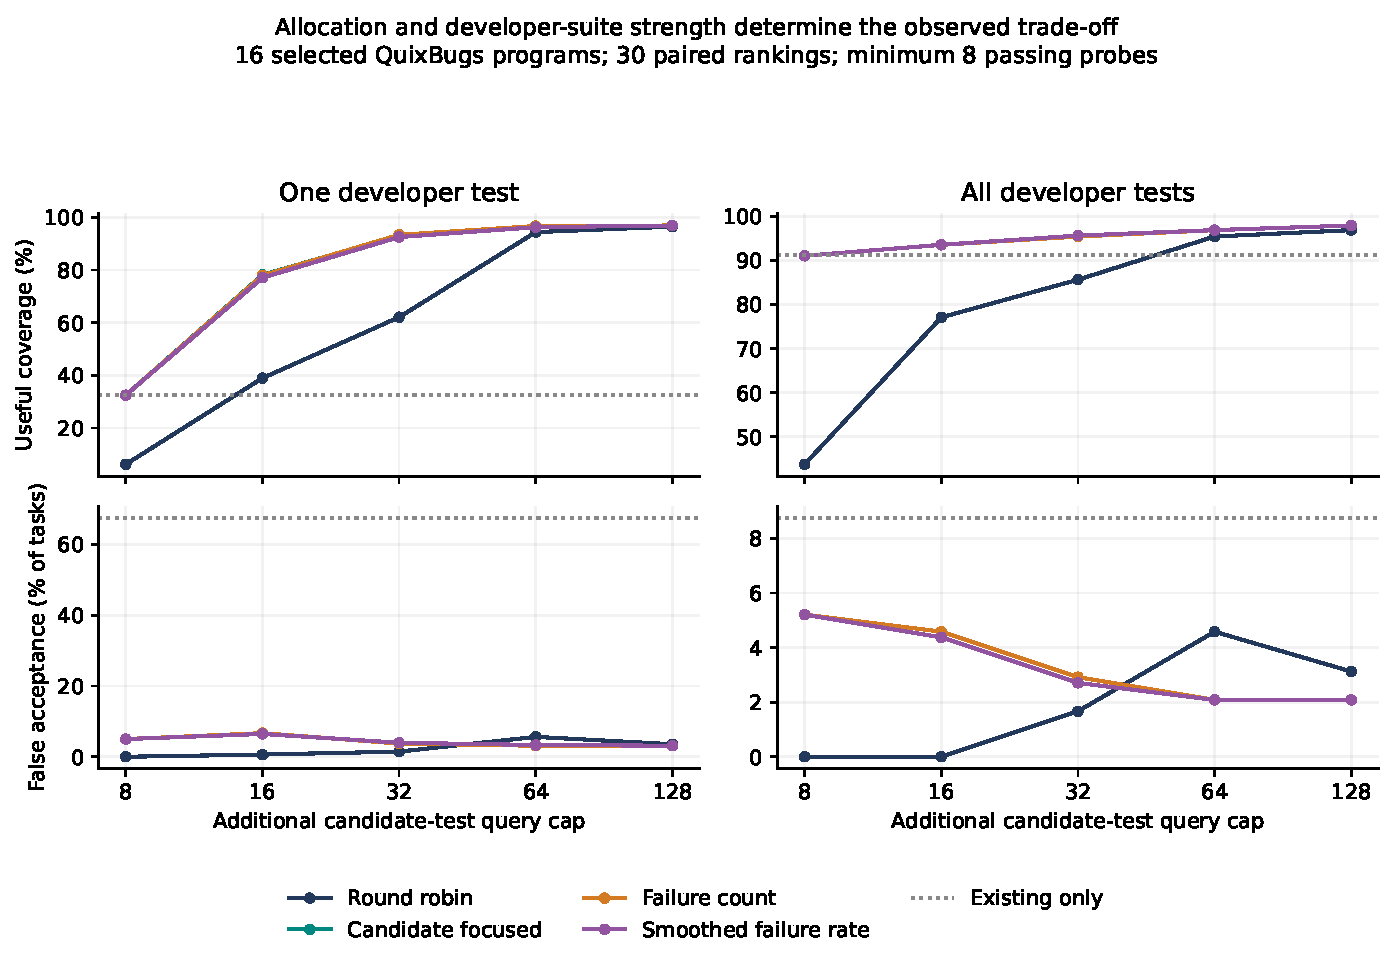
\includegraphics[width=\linewidth]{../figures/budget_tradeoff.pdf}
\caption{Budget sensitivity with minimum eight passing probes. The dashed reference uses only developer tests. Curves average 30 rankings per algorithm and then the 16 selected algorithms. The full machine-readable grid includes the three-test gate and all thresholds.}\label{fig:budget}
\end{figure}

Failure-count ordering reaches \FailureCountUseful\% useful coverage and \FailureCountFalse\% false acceptance in the primary setting. This baseline isolates one established use of failure history while keeping allocation and acceptance fixed. The complete results retain ties and unfavorable outcomes; no superiority over published full repair systems is implied. Figure~\ref{fig:budget} also makes developer-suite strength visible. When the gate already eliminates distinguishable variants, additional scheduling has less opportunity to improve held-out agreement.

\begin{figure}[t]
\centering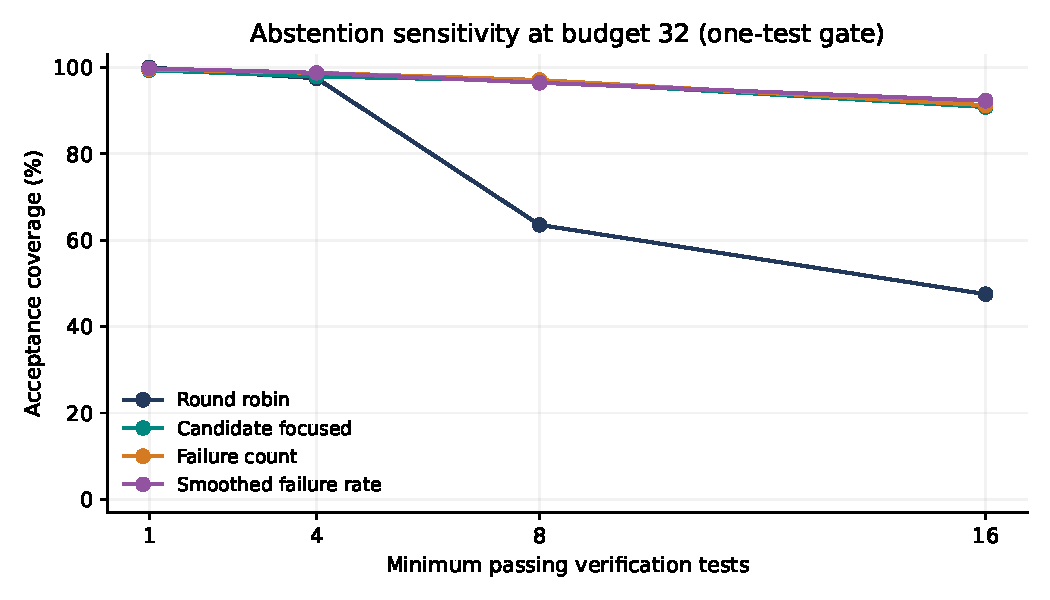
\includegraphics[width=0.85\linewidth]{../figures/threshold_ablation.pdf}
\caption{Acceptance-rule ablation. At a common query cap, raising the minimum evidence threshold can make broadly distributed testing abstain. This is an intended diagnostic of allocation and acceptance coupling.}\label{fig:threshold}
\end{figure}

The threshold ablation in Figure~\ref{fig:threshold} prevents interpreting abstention as a correctness improvement. A policy can lower false acceptance by selecting nothing; useful coverage and total coverage must be considered alongside conditional agreement. Similarly, the existing-only baseline spends fewer calls but does not satisfy the verification evidence threshold. Its point is to quantify the gate's initial screening strength, not provide an equal-information comparison.

\section{Discussion and limitations}
The observations support a narrow methodological conclusion: fixed-budget verifier evaluations must specify candidate allocation, acceptance thresholds, developer-suite strength, and oracle privileges together. Reported reliability without coverage can reward trivial abstention, and a query budget alone does not control runtime. A concentrated policy's coverage advantage can arise directly from the acceptance threshold even without better test ordering.

The fault model is artificial. Mutations of a known corrected program need not resemble plausible LLM repairs, and the planted reference ensures a solution is available. The inputs cover bounded, documented domains; finite agreement cannot identify semantic equivalence. Inputs are exact-disjoint but identically distributed, so the held-out pool does not evaluate distribution shift. Shared reference-oracle access excludes oracle hallucination, weak assertions, and specification ambiguity that real generated tests face. Independent specification implementations reduce a source of implementation error without proving the specification complete.

The algorithms are small and deterministic. We evaluate neither repositories nor flaky tests, integration setup, expensive model calls, parallel execution, or adversarial candidate code. Every query has unit logical cost despite large differences in execution time. Thirty ranking seeds explore order sensitivity but do not enlarge the corpus to 480 independent defects. Published FRTP, MPTPS, and CI systems solve related but different end-to-end tasks; only a transparent FRTP-inspired ordering is implemented here. There is no claim of state-of-the-art performance, established novelty, or publication readiness.

A stronger submission would require real fixed candidate-patch pools, independent test oracles unavailable to the solver, repository-level evaluation, meaningful cost models, and faithful relevant baselines. The current manuscript is a complete report of the scoped controlled experiment and a starting artifact for that work. It has not been submitted, accepted, or independently peer reviewed.

\section{Conclusion}
PatchBudget provides an auditable execution-based study of budgeted candidate screening. The protocol separates actual outcome collection from charged scheduling and discloses the effects of abstention, suite strength, and oracle access. The reported comparisons characterize this selected mutation corpus; extending them to autonomous program repair requires additional evidence.

\paragraph{AI assistance and authorship.}
AI tools assisted with literature review, study design, code, experiments, analysis, and manuscript drafting. The displayed author name is provided for the user's review; no institutional affiliation, supervisor involvement, coauthor endorsement, or independent human validation is asserted. The author must verify authorship and disclosure before external submission. No employer code, resume contact details, or historical project metrics are used as new evidence.

\bibliographystyle{plainnat}
\bibliography{references}
\appendix
\small
\section{Corpus inventory}
\begin{table}[h]
\centering\small\begin{tabular}{lrrrr}\toprule
Program & Candidates & Gate 1 & Gate all & Holdout pass\\\midrule
bitcount & 10 & 1 & 1 & 1\\
bucketsort & 9 & 6 & 1 & 1\\
find\_first\_in\_sorted & 24 & 10 & 5 & 2\\
gcd & 6 & 3 & 1 & 1\\
get\_factors & 16 & 13 & 2 & 4\\
is\_valid\_parenthesization & 17 & 3 & 1 & 1\\
knapsack & 23 & 8 & 5 & 4\\
kth & 10 & 2 & 2 & 2\\
lcs\_length & 14 & 4 & 1 & 1\\
lis & 24 & 22 & 3 & 2\\
max\_sublist\_sum & 9 & 6 & 2 & 2\\
mergesort & 23 & 23 & 2 & 2\\
next\_permutation & 25 & 8 & 5 & 2\\
quicksort & 11 & 4 & 2 & 2\\
sieve & 11 & 9 & 1 & 1\\
to\_base & 9 & 2 & 1 & 1\\
\bottomrule\end{tabular}

\caption{Candidate counts and gate survivors. Holdout pass counts agreement on all evaluation inputs before gate filtering. Equivalent mutants are intentionally retained.}\label{tab:inventory}
\end{table}

\section{Reproduction and evidence}
From the repository root, install the locked analysis dependencies and run:
\begin{verbatim}
python scripts/prepare.py
python -m unittest discover -s tests -v
python scripts/run.py --output reproduction/full
python scripts/verify.py --reproduction reproduction/full
python scripts/analyze.py
cd paper && tectonic main.tex
\end{verbatim}
\end{document}
